
\documentclass[xcolor=table]{beamer}

% for fancy Mike style table
 \usepackage[table]{xcolor} 
 \usepackage{multirow}
\usepackage{textpos}
\usepackage{helvet}
\usepackage{caption}
\usepackage{changepage}
\usepackage{algorithmic}
\usepackage{array}
\setbeamerfont{caption}{size = \footnotesize}
\usepackage{multicol}
\usepackage{setspace}

% useful packages for including code
\usepackage{listings}
\usepackage{color}
\lstset{breaklines}

% package for drawing graphs
\usepackage{tikz}
\usetikzlibrary{positioning}

\definecolor{charlesBlue}{RGB}{100, 155, 255}
\definecolor{charlesBlue2}{RGB}{0, 155, 255}
\definecolor{MRGGreen}{rgb}{0, 0.350, 0.200}
\usecolortheme{default}

% References
%\bibliographystyle{apacite} 
\hypersetup{colorlinks = true, linkcolor={MRGGreen}, citecolor = black, urlcolor = blue}


% Custom colors for alerts and examples
\setbeamercolor{palette primary}{fg=MRGGreen}
\setbeamercolor{palette secondary}{fg=MRGGreen}
\setbeamercolor{palette tertiary}{bg= MRGGreen}
\setbeamercolor*{structure}{fg=MRGGreen}
\setbeamercolor{titlelike}{fg=black}

\lstset{
  basicstyle=\tiny \ttfamily,
  columns=fullflexible,
}


\begin{document} 

\begin{frame}
  \begin{center}
    {\Large III} \\ \ \\ Ordinary differential equations in Stan
  \end{center}
\end{frame}

\begin{frame}
  \frametitle{Arsenal of tools}

  \begin{center}
    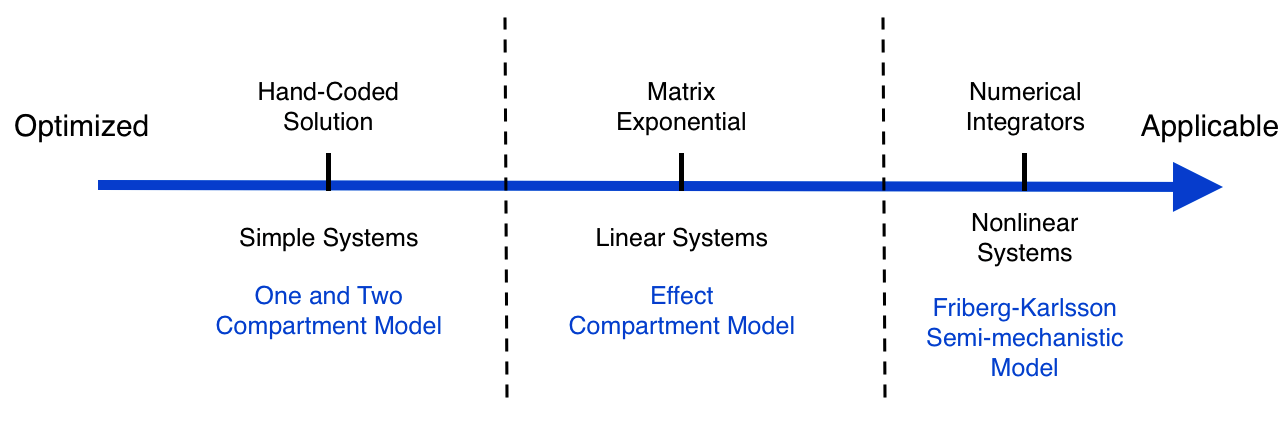
\includegraphics[width=4.5in]{../figures/odeSolvers.png}
  \end{center}

  For some examples, see \cite{Margossian:2017}.

\end{frame}

\begin{frame}

  \begin{itemize}
    \item the ``optimized - applicable'' spectrum is a heuristic; counter-examples can be built.
    \item coding effort may also be a criterion
  \end{itemize}

\end{frame}

\begin{frame}
  \frametitle{Matrix exponential}
  
  Consider a system of linear ODEs:
  $$ y^\prime(t) = Ky(t) $$
  where $K$ is a constant matrix.
  
  \ \\ Then
    $$ y(t) = e^{tK} y_0 $$

\end{frame}

\begin{frame}
  \frametitle{Matrix Exponential}
  
  $$ e^{tK} = \sum_{n=0}^{\infty} \dfrac{(tK)^n}{n!} = I + tK + \frac{(tK)^2}{2} + \frac{(tK)^3}{3!} + ... $$

\end{frame}

\begin{frame}
  \frametitle{Matrix Exponential}

  For example, the two compartment model generates the following matrix:
  \[ K = \begin{bmatrix}
       -ka & 0 & 0 \\
       ka & - (CL + Q) / Vc & Q / Vp \\
       0 & Q / V_c & - Q / V_p
     \end{bmatrix}
  \]
  
\end{frame}

\begin{frame}
  \frametitle{Linear ODE solver in Torsten}

    \texttt{
    pmx\_solve\_\textcolor{MRGGreen}{linode}(time, amt, rate, ii, evid, \\ 
    \hspace{3.3cm} cmt, addl, ss, \\
     \hspace{3.3cm} \textcolor{MRGGreen}{K}, biovar, tlag)
   }

\end{frame}

\begin{frame}
  \frametitle{Numerical integrators}

  Required for systems of nonlinear ODEs. \\ \ \\

  Stan supports three numerical integrators
  \begin{itemize}
    \item Runge-Kutta 4th/5th (rk45): non-stiff equations
    \item Adams-Moulton (am): non-stiff equations, scales better with number of steps
    \item Backward differentiation (bdf): stiff equations
  \end{itemize}
  
\end{frame}

\begin{frame}
  \frametitle{Numerical integrators}
  
  \ \\ \ \\
  
  \texttt{
    y = integrate\_ode\_rk45(system, y0, t0, ts, \\
    \hspace{4.5cm} theta, x\_r, x\_i);
  }
  
  \ \\ \ \\
  \begin{itemize}
    \item \texttt{system}: a function which returns $y' = f(y, t, \theta, x_r, x_i)$.
    \item \texttt{y0}: the initial condition at time \texttt{t0}.
    \item \texttt{t0}: the initial time
    \item \texttt{ts}: times at which we require a solution
    \item \texttt{theta}: parameters to be passed to \texttt{system()}.
    \item \texttt{x\_r}: real data to be passed to \texttt{system()}.
    \item \texttt{x\_i}: integer data to be passed to \texttt{system()}.
  \end{itemize}

\end{frame}

\begin{frame}
  \frametitle{Numerical integrators}
  
  Can also add tuning parameters for the ODE solvers:
  
  \ \\ \ \\
  
    \texttt{
    y = integrate\_ode\_rk45(system, y0, t0, ts, \\
    \hspace{4.5cm} theta, x\_r, x\_i \\
    \hspace{2.5cm} \textcolor{MRGGreen}{rel\_tol, abs\_tol, max\_num\_steps});
  }
  
  \ \\
  See chapter 21 of the Stan user manual. \\ \ \\
  The default values are 1e-6, 1e-6, and 1e+6, 
  but there are no theoretical justification for using these defaults.

\end{frame}

\begin{frame}
  \frametitle{System function}
  
  \begin{itemize}
    \item Declare system in the \texttt{functions} block.
  \end{itemize}
  
  \texttt{
    real[] system(real time, \\
    \hspace{2.8cm} real[] y, \\
    \hspace{2.8cm} real[] theta, \\
    \hspace{2.8cm} real[] x\_r, \\
    \hspace{2.8cm} int[] x\_i) \{ \\
    \ \ real[3] dydt; \\
    \ \ CL = theta[1]; \\
    \ \ Q = theta[2]; \\
    \ \ . \\ \ \ . \\ \ \ . \\
    \ \ return dydt; \\ \}
   % 
  }

\end{frame}

\begin{frame}
  \frametitle{Torsten function}
  
    \texttt{
  pmx\_solve\_rk45(system, nCmt, \\
  \hspace{2.9cm} time, amt, rate, ii, evid, \\ 
  \hspace{2.9cm} cmt, addl, ss, \\
  \hspace{2.9cm} theta, biovar, tlag, \\
  \hspace{2.9cm} rel\_tol, abs\_tol, max\_num\_steps)
  }

  \ \\ \ \\
  \textit{\textcolor{MRGGreen}{Exercise 3}: Write, fit, and diagnose the two compartment
  model using the \texttt{pmx\_solve\_rk45} function.}

\end{frame}

\begin{frame}
  \frametitle{Example: nonlinear ODE system}
  
  Consider the Friberg-Karlsson semi-mechanistic model \cite{Friberg:2002}.
  
  \begin{center}
    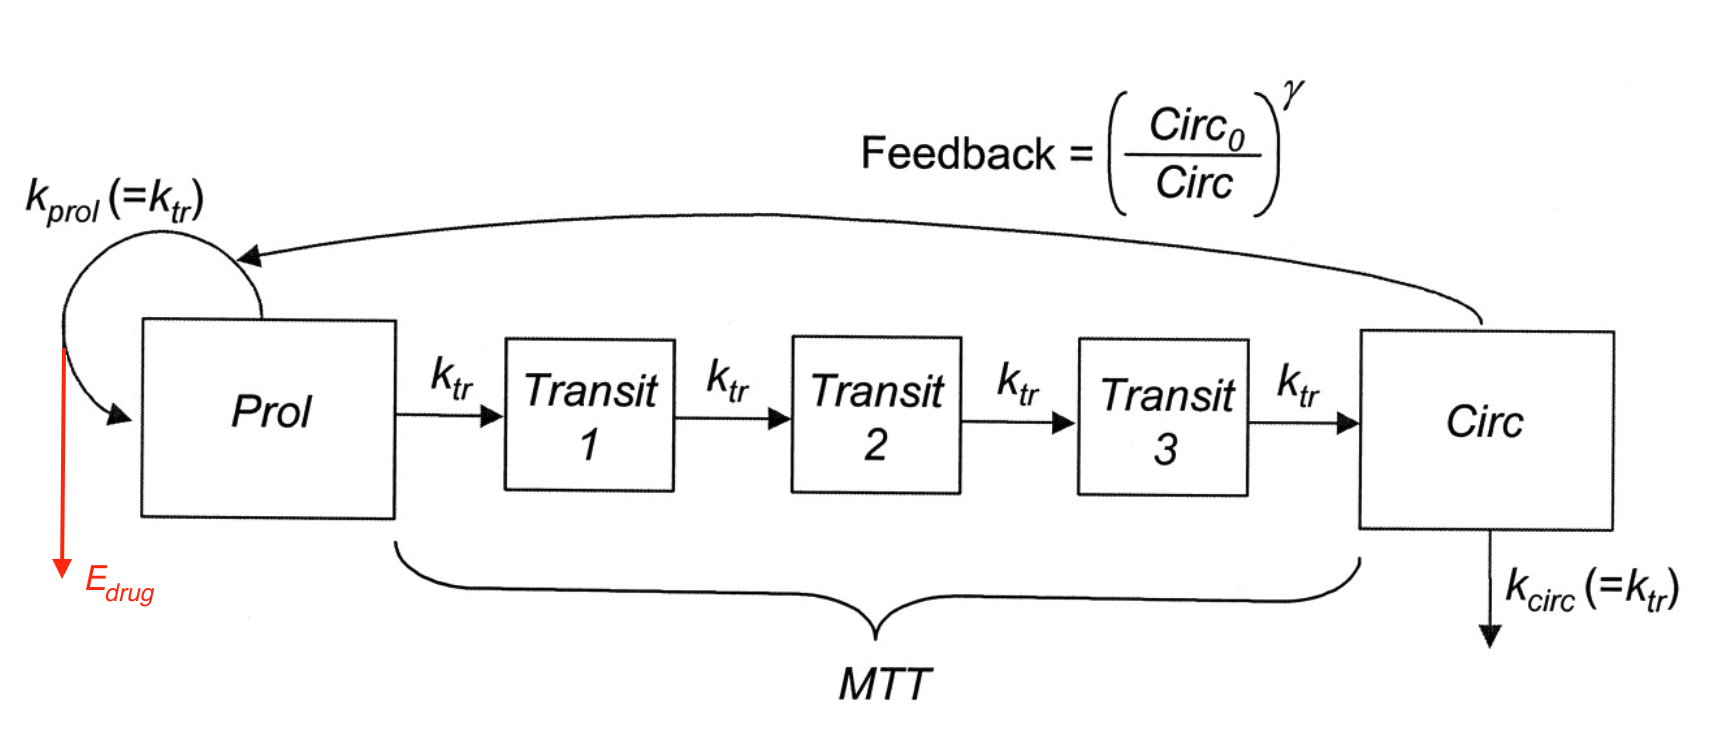
\includegraphics[width=8.5cm]{../figures/Friberg-Karlsson_drug}
  \end{center}

\end{frame}

\begin{frame}
  This process is described by the following ODEs:
  
  \begin{eqnarray*}
  \begin{aligned}
  y_{\mathrm{prol}}' &= k_{\mathrm{tr}} y_{\mathrm{prol}} (1 - {\color{red}E_{\mathrm{drug}}})\left(\frac{Circ_0}
    {y_{\mathrm{circ}}}\right)^\gamma - k_{\mathrm{tr}}y_{\mathrm{prol}} \\
  y_{\mathrm{tr1}}' &= k_{\mathrm{tr}} y_{\mathrm{prol}} - k_{\mathrm{tr}} y_{\mathrm{tr1}} \\
  y_{\mathrm{tr2}}' &= k_{\mathrm{tr}} y_{\mathrm{tr1}} - k_{\mathrm{tr}} y_{\mathrm{tr2}} \\
  y_{\mathrm{tr3}}' &= k_{\mathrm{tr}} y_{\mathrm{tr2}} - k_{\mathrm{tr}} y_{\mathrm{tr3}} \\
  y_{\mathrm{circ}}' &= k_{\mathrm{tr}} y_{\mathrm{tr3}} - k_{\mathrm{tr}} y_{\mathrm{circ}} 
  \end{aligned}
  \label{eq:FK}
\end{eqnarray*}

\ \\ \ \\
  where $E_\mathrm{drug} = \alpha \frac{y_{\mathrm{cent}}}{V_{\mathrm{cent}}}$,
  $ktr = 4 / MTT$,
  and $\alpha \approx 3e-4$.

\end{frame}

\begin{frame}

  \begin{itemize}
    \item $y_\mathrm{cent}$ is obtained from a two compartment model.
    \item Our PK/PD model therefore has a total of 8 equations.
    \item This problem can be solved using \texttt{pmx\_solve\_*}.
  \end{itemize}

\end{frame}

\begin{frame}

  Alternatively, we may elect to solve the PK ODEs \textcolor{MRGGreen}{analytically} 
  and the PD ODEs \textcolor{MRGGreen}{numerically}.
  \begin{itemize}
    \item This can yield some speedup, in particular for problems that require ODE solutions
      and sensitivities (e.g \cite{Margossian:2017b}).
%    \item This scheme can be applied twice when computing steady states, and
%    is probably most efficient there.
%    \item My guess is that we can construct examples where there is no speedup.
  \end{itemize}

\end{frame}

\begin{frame}
  \frametitle{Torsten function}
  
  \texttt{
  pmx\_solve\_\textcolor{MRGGreen}{twocpt}\_rk45(\textcolor{MRGGreen}{reduced\_system}, nOde, \\
  \hspace{4.3cm} time, amt, rate, ii, evid, \\ 
  \hspace{4.3cm} cmt, addl, ss, \\
  \hspace{4.3cm} theta, biovar, tlag, \\
  \hspace{4.3cm} rel\_tol, abs\_tol, \\
  \hspace{4.3cm} max\_num\_steps)
  }
  
  \ \\ \ \\
  \begin{itemize}
    \item we now pass a ``reduced system''.
    \item we specify the number of ODEs to be solved numerically, not
    the number of compartments.
  \end{itemize}

\end{frame}

\begin{frame}

  \begin{itemize}
    \item \texttt{theta} now contains the parameters for the two cpt model, followed
    by the parameters that get passed to the numerical solver.
  \end{itemize}
  
  E.g: \\
   $$ \theta = \{CL, Q, VC, VP, ka, ...\} $$

\end{frame}

\begin{frame}
  The reduced system is: \\ \ \\
  
    \texttt{
    real[] reduced\_system(real time, \\
    \hspace{4.4cm} real[] y, \\
    \hspace{4.4cm} \textcolor{MRGGreen}{real[] yPK}, \\
    \hspace{4.4cm} real[] theta, \\
    \hspace{4.4cm} real[] x\_r, \\
    \hspace{4.4cm} int[] x\_i) \{ \\
    \ \ real[3] dydt; \\
    \ \ . \\ \ \ . \\ \ \ . \\
    \ \ return dydt; \\ \}
   % 
  }

\end{frame}

\begin{frame}

\textit{\textcolor{MRGGreen}{Exercise 4 (optional)}: Write, fit, and diagnose a Friberg-Karlsson model
with a two compartment with first order absorption PK. Use \texttt{FKModel.r}
and \texttt{data/FKModel.data.r}.} 

\end{frame}

\begin{frame}

\begin{itemize}
  \item You may either use \texttt{pmx\_solve\_*} or \texttt{pmx\_solve\_twocpt\_*}.
  \item Use $\alpha = 3e-4$ and estimate all other 8 ODE coefficients,
  i.e. $\theta = \{ CL, Q, VC, VP, ka, MTT, circ0, \gamma \}$.
  \item The initial state for the neutrophil count is $Circ_0$. 
  Either edit the event schedule to reflect this at time 0, 
  or write the solution to your ODEs as a deviation from the baseline.
 \end{itemize}

\end{frame}

\begin{frame}

  \begin{itemize}
    \item This exercise entails a few subtleties; in the interest of time we won't
    go through it in class.
    \item Here are however results I get from 3 chains with 500 iterations you can
    use as a benchmark.
  \end{itemize}

\end{frame}

\begin{frame}

  \begin{center}
    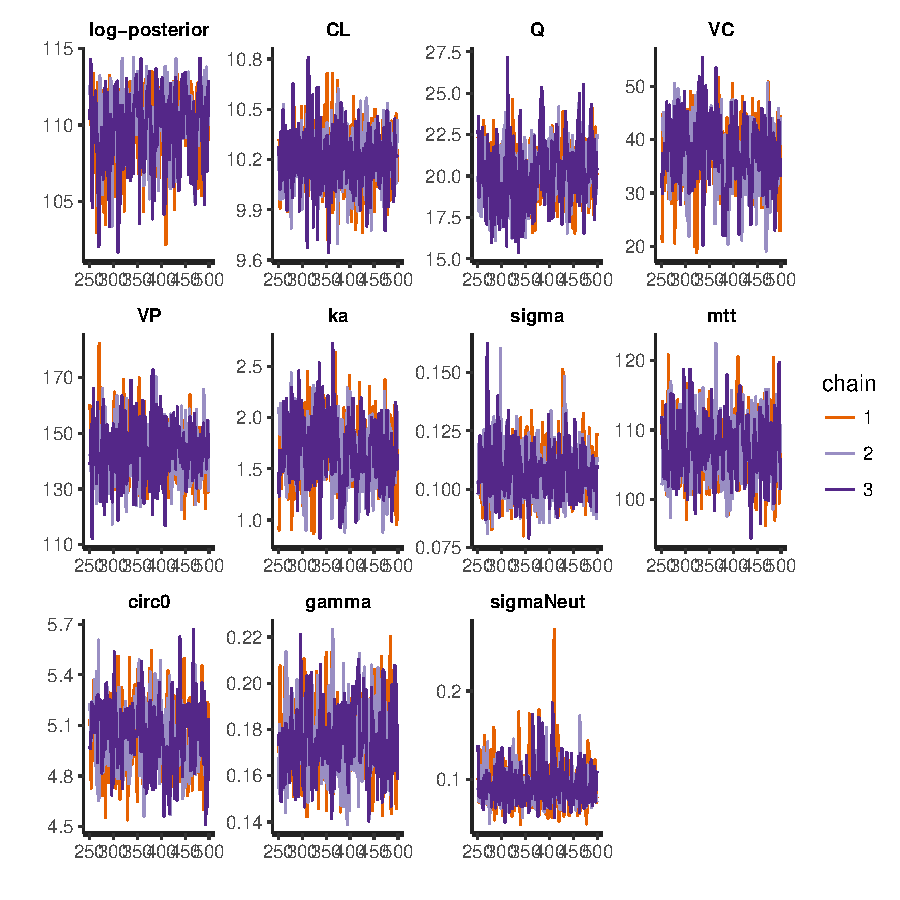
\includegraphics[width=7cm]{../figures/FKModelPlots002.pdf}
  \end{center}

\end{frame}

\begin{frame}

  \begin{center}
    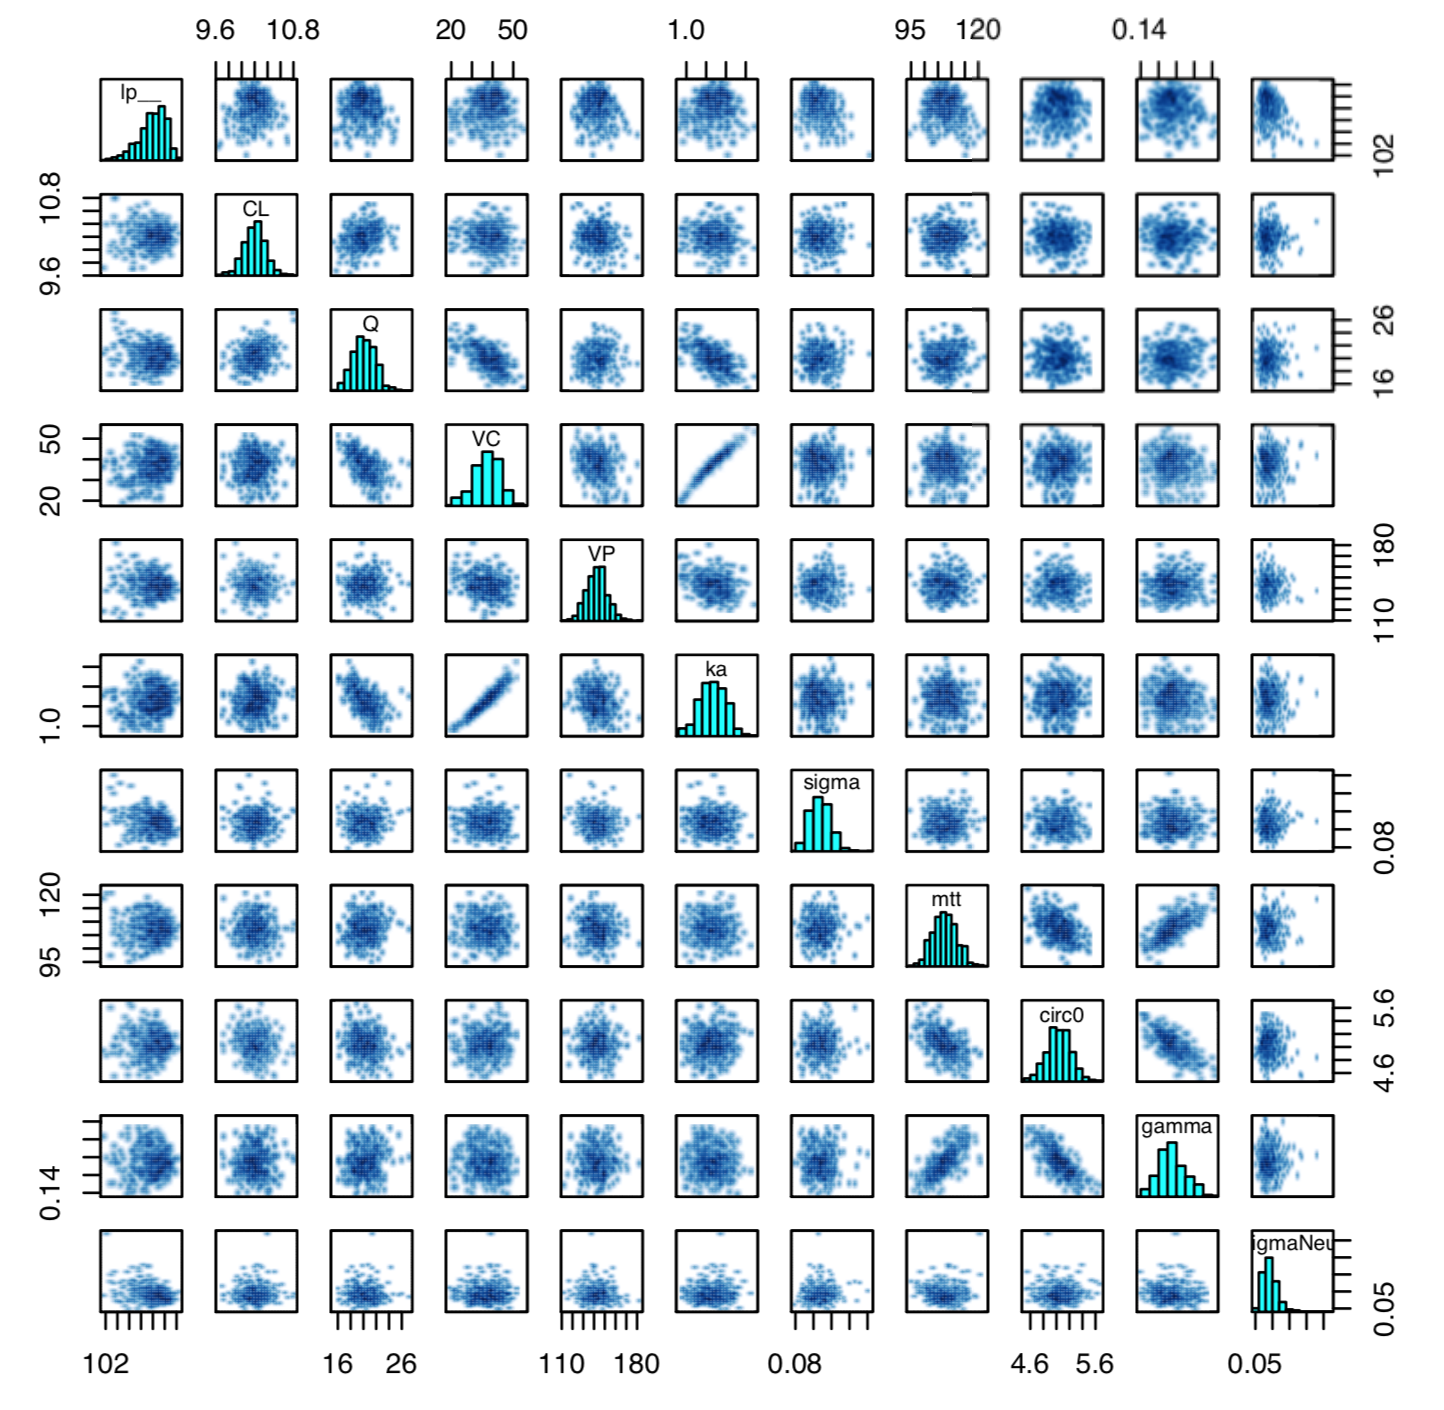
\includegraphics[width=7cm]{../figures/FKPairs}
  \end{center}

\end{frame}

\begin{frame}

  \begin{center}
    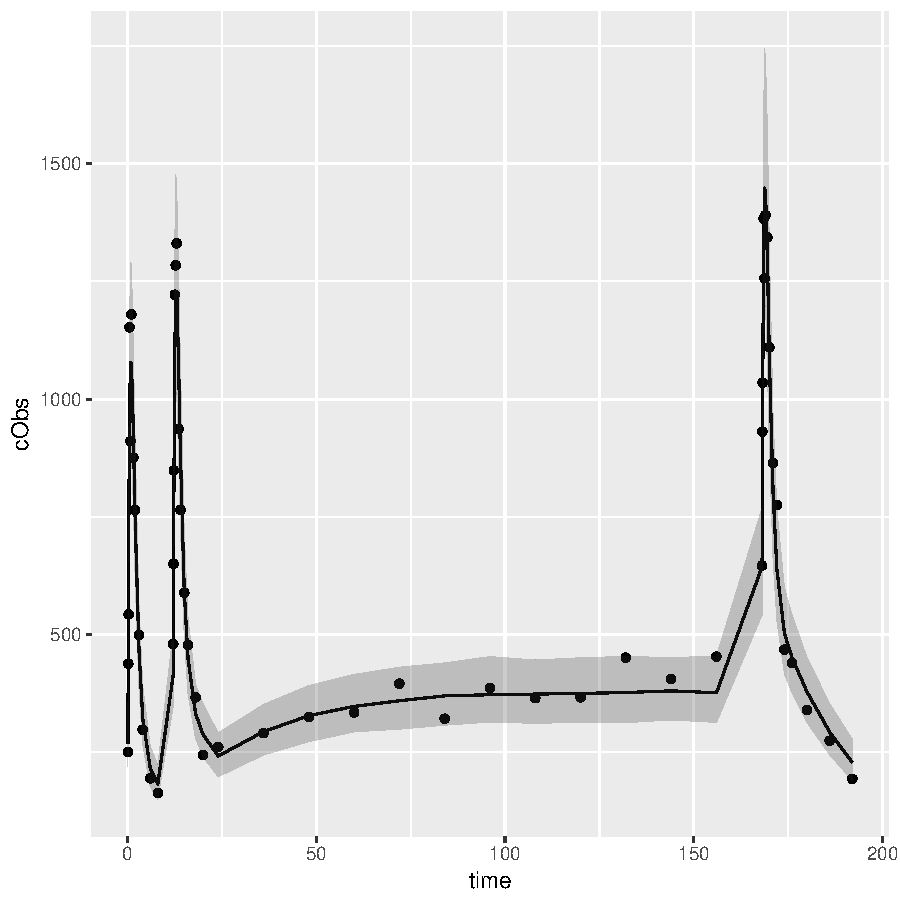
\includegraphics[width=7cm]{../figures/FKModelPlots005.pdf}
  \end{center}

\end{frame}

\begin{frame}

  \begin{center}
    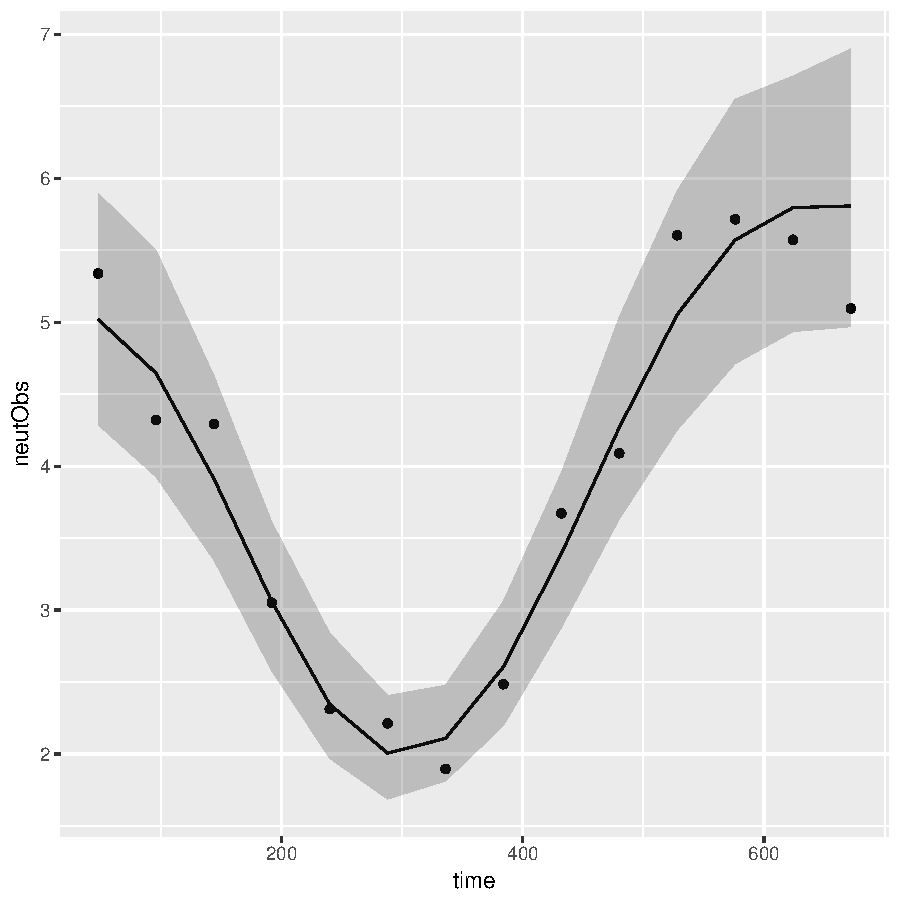
\includegraphics[width=7cm]{../figures/FKModelPlots006.pdf}
  \end{center}

\end{frame}

\section{References}
\begin{frame}[allowframebreaks]{References}
\scriptsize
% \bibliographystyle{unsrt}
%\bibliographystyle{authoryear}
\bibliographystyle{apalike}
\bibliography{../ref}  
\end{frame}

\end{document}
